\documentclass{boi2014-lv}
%\setdefaultlanguage{latvian}

\usepackage{enumitem}
\usepackage{wrapfig}
\usepackage{mathtools}
\usepackage{tikz}

\renewcommand{\DayNum}{1}
\renewcommand{\TaskCode}{coprobber}
\renewcommand{\TaskName}{Policists un zaglis}

\renewcommand{\labelitemii}{$\circ$}
\newcommand{\constant}[1]{{\tt #1}}

\begin{document}
    \begin{wrapfigure}[8]{r}{6cm}
        \vspace{-24pt}
		\includegraphics[width=6cm]{\TaskCode.jpeg}
	\end{wrapfigure}

	Baitimorā noziedzības līmenis ir sasniedzis visu laiku augstāko līmeni. Zādzības notiek katru dienu. Kad noziegums ir izdarīts, patrulējošajam policistam vienam pašam ir jāķer zaglis pa šaurajām ielām un krustojumiem, kas savieno ielas. Diemžēl zagļiem biežāk izdodas aizbēgt no policistiem, nekā tie tiek noķerti, jo zagļi pārzina pilsētu daudz labāk nekā policija.
   % In the city of Bytemore crime level is hitting an all--time high.
    %Among other misdemeanours, robberies are happening every day.
    %And when the crime is committed, it is always up to a lone patrolling
    %police officer to chase down the robber through the narrow alleys
    %that connect street corners (commonly referred to simply as
    %\emph{corners}). Unfortunately, more often than not, robbers escape
    %their pursuers, because they know the city much better than
    %the police.

	Baitimoras pilsētas policijas departaments (BPPD) organizē sanāksmi, lai samazinātu noziedzību. Viena no iniciatīvām ir izmantot datoru zagļu ķeršanai. Šim nolūkam BPPD ir izveidojis precīzu pilsētas karti un tagad viņiem tikai nepieciešama programmatūra, kas atradīs ķeršanas stratē\v{g}ijas.

   % The Bytemore City Police Department (BCPD) is organising a summit
    %to reduce crime. One of the initiatives is to use computer aid when
    %pursuing the robbers. For this purpose, the BCPD has made a precise
    %map of the city. Now they need computer software to find chasing
    %strategies.

    %The pursuit problem of one officer chasing one robber is modelled
    %as follows:
	Pakaļdzīšanās, kad viens policists ķer vienu zagli tiek modelēta šādā veidā:
    \begin{enumerate}
        \item Policists izvēlas krustojumu kurā patrulēt
	%The police officer chooses a corner on which to patrol.
        \item Zaglis izvēlas krustojumu, kurā veikt zādzību (viņš zina policista atrašanās vietu). No šī brīža tiek pieņemts, ka gan policists gan zaglis zina otra atrašanās vietu.
	%The robber then chooses a corner for the robbery
            %(he knows where the officer is). From this moment on it
            %is always assumed that both the officer and the robber
            %know where each other is.
        \item Policista gājiena laikā viņš pārvietojas uz kādu no kaimiņu krustojumiem (t.i. krustojumiem kuros var nokļūt no pašreizejā krustojuma ejot pa ielu) vai ari gaida (t.i. nekur neiet).
	%The police officer's move consists of him moving to a
            %neighbouring corner (i.e. one that is connected to the
            %current one by an alley) or waiting (i.e. not moving).
        \item Zagļa gājiena laikā viņš pārvietojas uz kādu no kaimiņu krustojumiem. Ievērjoiet, ka atškirībā no policista, zaglis nevar gaidīt, jo viņu instinkti liek tiem turpināt skriet.
	%The robber's move consists of him moving to a neighbouring
            %corner. Note that, unlike the police, robbers cannot wait.
            %It is in their instinct to keep running.
        \item Policists un zaglis pārmaiņus izdara gājienus (policists sāk pirmais), kamēr iestājas viens no šiem gadījumiem:
	%The police officer and the robber keep making moves one after
        %another (starting with the officer) until one of the following
        %happens:
        \begin{enumerate}
            \item situācija atkārtojas (situācija tiek definēta kā policista un zagļa pozīcija un tas kuram nākamajam jāizdara gājiens).  Ja situācija atkārtojas, tad zaglis var izvairities no policista bezgalīgi ilgi un tātad viņš aizbēg.
	%situation repeats itself (situation is defined
                %by the positions of both agents and the side whose turn
               % it is to move next). This corresponds to the robber being
                %able to avoid the police officer indefinitely, so the
                %robber escapes;
            \item pēc policista vai zagļa gājiena abi nonāk vienā un tajā pašā krustojumā. Šajā gadījumā policists noķer zagli.
	%the police officer and the robber meet on the same corner
                %after a move of either of them. In this case the police officer
                %catches the robber.
        \end{enumerate}
    \end{enumerate}

    \Task
	Jums jāuzraksta programma, kas dotai pilsētas kartei noteiktu vai iespējams noķert zagli un ja tas ir iespējams, tad noķertu zagli, izdarot gajienus policista vietā.
   % You have to write a program which, given the map of the city,
    %would determine whether catching the robber is possible, and if it is,
    %would catch him by making moves on behalf of the police officer.

	Uzskatiet, ka zaglis izdara gājienus optimāli.
   % Your program must assume that the robber moves optimally.

    \Implementation
	Jums jārealizē divas funkcijas:
    %You need to implement two functions:
    \begin{itemize}
        \item funkcija \method{start(N, A)}, ar parametriem:
		%\method{start(N, A)} which takes the following parameters:
            \begin{itemize}
                \item $N$ --- krustojumu skaits (krustojumi sanumurēti no $0$ līdz $N-1$);%the number of corners (corners are labelled from $0$ to $N-1$);
                \item $A$ --- divdimensionāls masīvs, kas apraksta ielas $0 \le i, j \le N-1$%a two--dimensional array that describes the alleys: for $0 \le i, j \le N-1$,
                    $$
                        A[i, j] \text{ ir }
                        \begin{dcases*}
                            \texttt{false} & ja $i$ un $j$ nav savienoti ar ielu
                                \\
                            \texttt{true} & ja $i$ un $j$ ir savienoti ar ielu
                        \end{dcases*}
                    $$
		Visas ielas ir divvirzienu (t.i.  $A[i, j] = A[j, i]$ visiem $i$ un $j$) un nav tādu ielu, kas sākas vienā un tajā pašā krustojumā (t.i. $A[i, i]$ būs \texttt{false} visiem $i$). Jūs varat pieņemt, ka no jebkura krustojuma, pārvietojoties pa ielām, būs iespējms nokļūt jebkurā citā krustojumā.
                   % All alleys will be bidirectional (i.e. $A[i, j] = A[j, i]$
                    %for all values of $i$ and $j$) and there will be no alleys
                    %connecting a corner to itself (i.e.  $A[i, i]$ will be
                    %\texttt{false} for all values of $i$).  Also, you may assume
                    %that it will always be possible to reach any corner from any
                    %other corner by moving along the alleys.
            \end{itemize}

	Ja parametros aprakstītajā kartē ir iespējams noķert zagli, tad funkcijai \method{start} jāatgriež tā krustojuma numurs uz kura policists izvēlas patrulēt. Citādi jāatgriež $-1$.
       % If it is possible to catch the robber on the map described
        %by the parameters, function \method{start} should return the
        %label of the corner on which the police officer chooses to patrol.
        %Otherwise, it should return $-1$.

        \item funkcija \method{nextMove(R)}, kas parametrā saņem krustojuma numuru $R$, kurā pašlaik atrodas zaglis, un funkcijai jāatgriež tā krustojuma numuru, kurā atradīsies policists pēc sava gājiena izdarīšanas.
	%which takes as a
            %parameter the label $R$ of the current corner of the robber
            %and must return the label of the corner where the officer
            %will be after his move.
    \end{itemize}

	Funkcija \method{start} tiks izsaukta tieši vienu reizi pirms funkcijas \method{nextMove} izsaukšanas. Ja funkcija \method{start} atgriež $-1$, tad funkcija \method{nextMove} netiks izsaukta, bet citos gadījumos funkciju \method{nextMove} izsauks tikmēr kamēr pakaļdzīšanās beigsies. Precīzāk, programma pārtrauks darbu tiklīdz izpildīsies viens no sekojošiem nosacījumiem:
   % Function \method{start} will be called exactly once before any
    %calls to \method{nextMove} are made. If \method{start} returns
    %$-1$, then \method{nextMove} will not be called. Otherwise,
    %\method{nextMove} will be called repeatedly until the pursuit ends.
    %More precisely, the program will terminate as soon as one of the
    %following happens:
    \begin{itemize}
        \item funkcija \method{nextMove} atgriež nekorektu gājienu;%\method{nextMove} returns an invalid move;
        \item situācija atkārtojas;%the situation repeats itself;
        \item zaglis tiek noķerts.%the robber is caught.
    \end{itemize}

    \Example
    \begin{wrapfigure}[4]{r}{2cm}
        \vspace{-0.5cm}
        \centering
        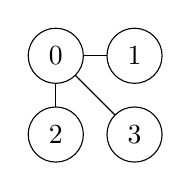
\begin{tikzpicture}
        \draw (0,1) -- (0,0);
        \draw (0,1) -- (1,0);
        \draw (0,1) -- (1,1);
        \foreach \x in {0,1} \foreach \y in {0,1}
            \draw (\x,\y) node[circle,draw,fill=white,inner sep=0,minimum size=0.7cm] {\pgfmathparse{int(2-2*\y+\x)}\pgfmathresult};
        \end{tikzpicture}
    \end{wrapfigure}
	Aplūkosim labajā pusē ilustrēto piemēru. Šajā gadījumā policistam jebkurš no krustojumiem ir laba sākuma pozīcija. Ja policists sāk patrulēt krustojumā 0, viņš var gaidīt un zaglis viņam uzskries virsū. Taču, ja policists sāk patrulēt jebkurā citā krustojumā, tad viņš var gaidīt kamēr zaglis nonāk krustojumā 0 un tad doties uz turieni.
    %Let's take a look at the example illustrated on the right. In this case any
    %corner is a good starting position for the police officer. If he starts in the
    %corner 0, he can wait in his first move and the robber will run into him.
    %On the other hand, if he starts on any other corner, he can wait until the
    %robber moves to corner 0, and then move there.
    
   % Here's how a sample session could look like:
	Šādi varētu izskatīties piemēra izpilde.

    \begin{tabular}{|l|c|}
        \hline
            {\bf Funkcijas izsaukums} & {\bf Rezultā\newline ts} \\
        \hline
            \method{start(4, [[0, 1, 1, 1], [1, 0, 0, 0], [1, 0, 0, 0], [1, 0, 0, 0]])} &
            \constant{3} \\
        \hline
            \method{nextMove(1)} & \constant{3} \\
        \hline
            \method{nextMove(0)} & \constant{0} \\
        \hline
    \end{tabular}

	Piezīme: īsākam pierakstam iepriekš aprakstītajā funkcijas \method{start} izsaukumā \constant{0} apzīmē \constant{false} un \constant{1} apzīmē \constant{true}.

    %Note: in the call to \method{start} above \constant{0} zero denotes
    %\constant{false} and \constant{1} denotes \constant{true} for brevity.

    \Scoring
    %In order to score full points, your solution must:
	Lai iegūtu punktus Jūsu risinājumam jāspēj:
    \begin{enumerate}
    	\item korekti noteikt vai policists var noķert zagli;%correctly determine whether the police officer can catch
    		%the robber;
	\item izpildot gājienus policista vietā noķert zagli.%successfully catch the robber by making moves on behalf
		%of the police officer.
    \end{enumerate}
    
	Apakšuzdevumiem 3 un 4 risinājumi, kas izpilda tikai pirmo nosacījumu iegūs 30\% no apakšuzdevuma punktiem.
    %However, in subtasks 3 and 4, solutions that only implement the
    %first requirement will score 30\% subtask points. 

    \begin{description}
        \item[Apakšuzdevums 1 (16 punkti):] $2 \le N \le 500$. Starp katriem diviem krustojumiem ir tieši viens ceļš.%There will be exactly one path between every pair of corners.
        \item[Apakšuzdevums 2 (14 punkti):] $2 \le N \le 500$.  Krustojumu un ielu tīkls veidos rež\v{g}veida strutūru. Rež\v{g}im būs vismaz divas rindas un kolonnas un krustojumu numerācija atbildīs zemāk norādītajam šablonam.
        %The network of corners
        %and alleys will form a grid-shaped structure. The grid will have at
        %least two rows and columns and the street corner labelling will follow
        %the pattern illustrated below.
        \begin{figure}[h!]
           \centering
           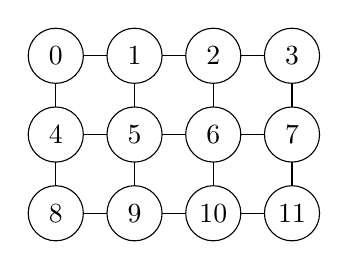
\begin{tikzpicture}
            \draw (0,0) grid (3,2);
            \foreach \x in {0,1,2,3} \foreach \y in {0,1,2}
                \draw (\x,\y) node[circle,draw,fill=white,inner sep=0,minimum size=0.7cm] {\pgfmathparse{int(8-4*\y+\x)}\pgfmathresult};
           \end{tikzpicture}
        \end{figure}
        \item[Apakšuzdevums 3 (30 punkti):] $2 \le N \le 100$.
        \item[Apakšuzdevums 4 (40 punkti):] $2 \le N \le 500$.
    \end{description}

    \Constraints
    
    \begin{description}
        \item[Laika ierobežojums:] 1 s.
        \item[Atmiņas ierobežojums:] 256 MB.
    \end{description}

    \Experimentation
    
	Pārbaudes programma uz Jūsu datora lasīs ievaddatus no standarta ievada. Pirmajā ievaddatu rindā jābut naturālam skaitlim $N$ --- krustojumu skaitam. Nākamajās $N$ rindām jāsatur kaimiņu matricu $A$, katrā no rindām jābūt $N$ skaitļiem, kur katrs ir vai nu 0 vai 1. Matricai jābūt simetriskai un uz galvenās diagonāles jābūt nullēm. 
%	The sample grader on your computer will read data from the standard input.
%    The first line of the input should contain integer $N$ --- the number of
%    corners.  The following $N$ lines should contain the adjacency matrix $A$.
%    Each of these lines should contain $N$ numbers, where each one is 0 or 1.
%    The matrix must be symmetric and the main diagonal values must all be
%    zeroes.

	Nākamajai rindai jāsatur skaitlis 1, ja policists var noķert zagli, bet 0 citos gadijumos.
%    The next line should contain number 1, if police can catch the robber,
%    and 0 otherwise.

	Ja policists var noķert zagli, tad jābūt vēl $N$ rindām, kas apraksta zagļa stratē\v{g}iju. Katrai no šīm $N$ rindām jāsatur $N+1$ vesels skaitlis ar vērtību no 0 līdz $N-1$. $r$-tās rindas $c$-tās kolonnas, kur $c < N$, vērtība apraksta uz kurieni dosies zaglis, savā gājienā ja policists atrodas krustojumā $r$, bet zaglis --- krustojumā $c$. Vērtības uz galvenās diagonāles tiks ignorētas, jo tās atbilst situācijām, kad zaglis un policists ir vienā un tajā pašā krustojumā. Labējā kolonna norāda kurā vietā sāks zaglis atbilstoši katrai policista izvēlētajai sākuma pozīcijai.
%    Finally, if police officer can catch the robber, $N$ lines should follow,
%    describing the strategy of the robber.  Each of these lines should contain
%    $N+1$ integers between 0 and $N-1$.  The value at row $r$ and column $c$,
%    where $c < N$, corresponds to a situation where it's robber's turn, the
%    police officer is at corner $r$ and the robber is at corner $c$, and
%    represents the corner, which the robber has to move to.  The main diagonal
%    values will be ignored, as they correspond to situations where the robber
%    and the police officer are at the same corner.  The right--most column
%    defines robber's starting corners for each possible police officer's
%    starting corner.

	Šeit redzams, kā pārbaudes programmai aprakstītu piemēru ar trim krustojumiem, kas savienoti savā starpā.
%    Here is an example input to the sample grader which represents three corners
%    that are connected together:
	

    \begin{center}
        \begin{tabular}{p{4cm}}
            {\tt
                3 \newline
                0 1 1 \newline
                1 0 1 \newline
                1 1 0 \newline
                1 \newline
                0 2 1 2 \newline
                2 0 0 2 \newline
                1 0 0 1 \newline
            }
        \end{tabular}
    \end{center}

	Šeit doti ievaddati, kas atbilst uzdevuma formulējumā dotajam piemēram.
    %And here is the input which matches the example given in the task statement
    %above:

    \begin{center}
        \begin{tabular}{p{4cm}}
            {\tt
                4 \newline
                0 1 1 1 \newline
                1 0 0 0 \newline
                1 0 0 0 \newline
                1 0 0 0 \newline
                1 \newline
                0 0 0 0 1 \newline
                2 0 0 0 2 \newline
                3 0 0 0 3 \newline
                1 0 0 0 1 \newline
            }
        \end{tabular}
    \end{center}
\end{document}
